\input{"./2ProjectSetup".tex}%
\input{"\DenKrLayoutMainRootDir/2includes/packages/preamble_pre".tex}%
\documentclass[tikz,fontsize=11pt,class=scrbook]{standalone}% I.e. the content from \input{"\DenKrLayoutMainRootDir/2layout/tikz_standalone/preamble_1_class".tex}%
\input{"\DenKrLayoutBaseRootDir/tikz_standalone/1TikzStandalonePicIncludeThis".tex}%
\DenKrTikzStandalonePre%
%
%
%
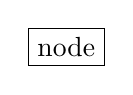
\begin{tikzpicture}[
	scale = 1.0,%Könnte das Makro \tikzpicturescale sein. Siehe in makros.tex
	% (Sollte eigentlich übergeben werden)(Beachte Möglichkeiten der Übergabe;
	% standalone mode=tex vs mode=buildnew)
	auto,
	node distance=\nodedistance
]
%
\node(p_a)%
    [draw]%
    {node};%
%
\end{tikzpicture}%
%
%
\DenKrTikzStandalonePost%